\section*{Possible appendices topics}

Hello, World.

\begin{figure}[h]
	\centering
	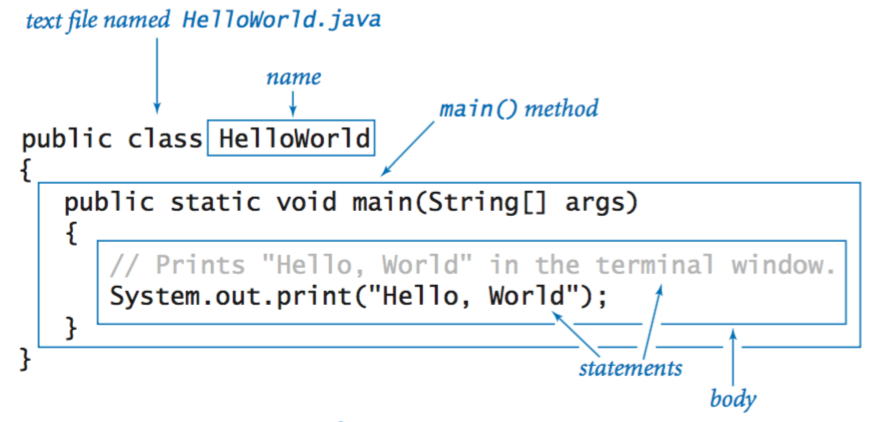
\includegraphics[width=0.85\textwidth]{images/hello_world_description}
	\label{fig:hello_world_description}
\end{figure}

Edit, compile, execute

\begin{figure}[h]
	\centering
	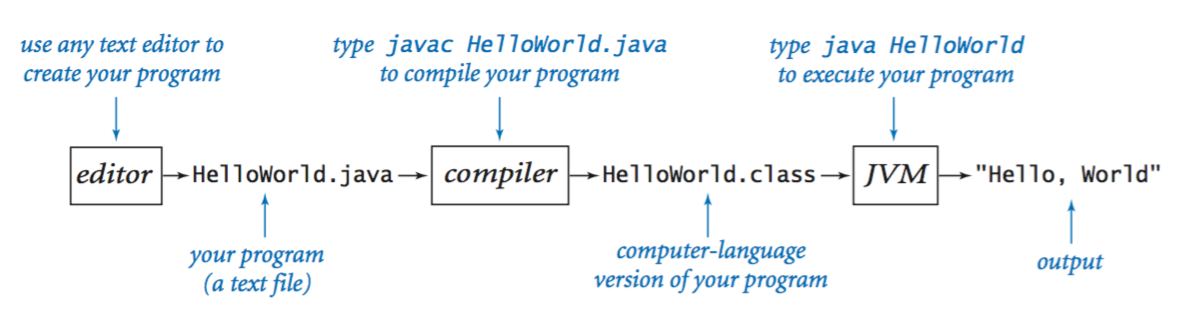
\includegraphics[width=0.85\textwidth]{images/edit_compile_execute}
	\label{fig:edit_compile_execute}
\end{figure}

Built-in data types

\begin{figure}[h]
	\centering
	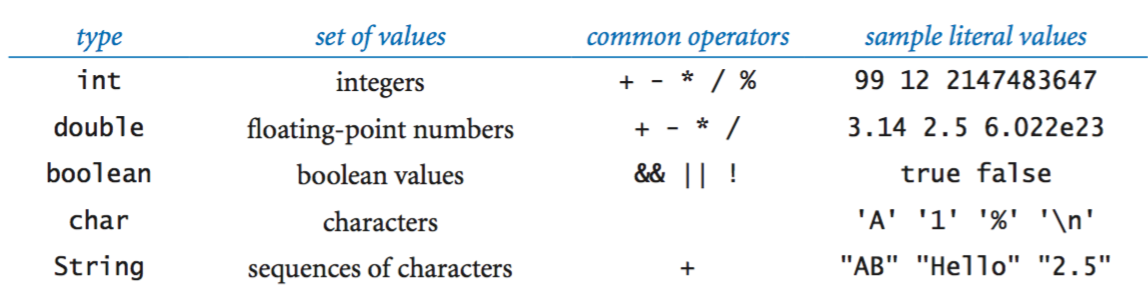
\includegraphics[width=0.85\textwidth]{images/data_types}
	\label{fig:data_types}
\end{figure}

Booleans

\begin{figure}[h]
	\centering
	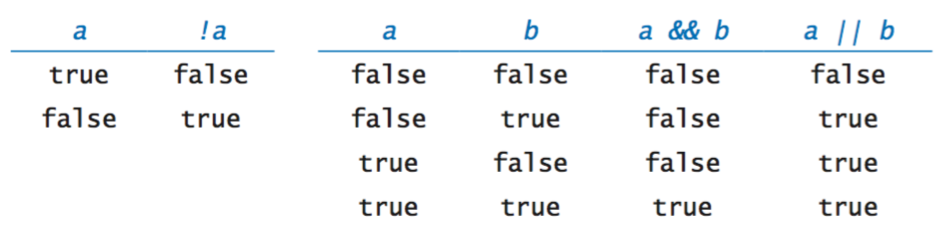
\includegraphics[width=0.85\textwidth]{images/booleans}
	\label{fig:booleans}
\end{figure}

Printing

System.out.print() is for regular printing
System.out.println() is same as System.out.print() but adds a newline
System.out.printf() prints \textbf{f}ormatted text, so you can easily insert data types inside a string and specify things like how many decimals should go after numbers. 
\begin{tabular}{|l|l|}
\hline
Format Specifier & Effect\\
\hline
\%s,\%S & Formats String\\
\%f & Formats floating point (precision provided between \% and f)\\
\%d & Formats integer\\
\%c & Formats character\\
\%b, \%B & Formats Boolean\\
\hline
\end{tabular}

Example: 

\begin{code}
System.out.printf("%.3f\n%.4f%d\n", 1.252525, 1.353535, 3);
\end{code}

prints 

\begin{code}
1.253
1.35353
\end{code}

\ja{todo: Scanners}

\ja{Cite https://introcs.cs.princeton.edu/java/11cheatsheet/}

\begin{itemize}

	\item Comparing floating point numbers.
	\item Type conversion.
	\item Useful math functions, e.g. \ic{min()}, \ic{log}.

\end{itemize}

\section{Java Reserved Words}

TODO: fill this in